\documentclass[aspectratio=169]{beamer}
\usepackage{framed}
\usepackage{lphs}
\usepackage{pifont}

\SetupImages{L2-Images/}{jpg}
\begin{document}

\section{Что такое деконструкция?}

\begin{Person}{deMan}{Поль де Ман}{1919 -- 1983}
\Citation{
Из опыта чтения абстрактных философских текстов нам всем знакомо облегчение, которое мы чувствуем, когда рассуждение сменяется тем, что называется <<конкретным примером>>. Однако именно в этот самый момент, когда нам наконец кажется, что мы все поняли --- мы, в действительности, дальше от понимания, чем когда-либо прежде}{}
\end{Person}

\begin{frame}
\begin{center}
\begin{tikzpicture}[x=3cm,y=-0.9cm]
\uncover<+->{\node at (-1,-1) {
\includegraphics[angle=10, width=7cm]{L2-Images/nose1.jpg}};}
\uncover<+->{\node at (1,-1) {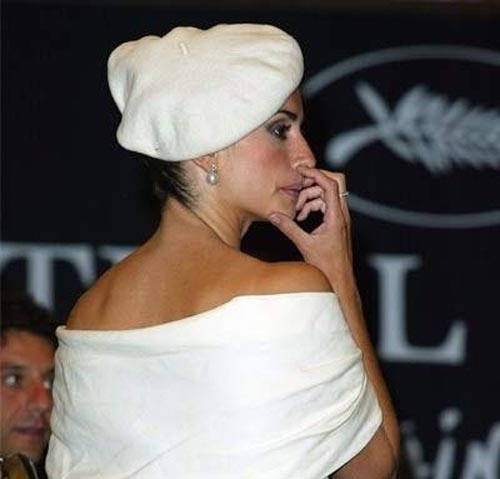
\includegraphics[angle=-5, width=7cm]{L2-Images/nose3.jpg}};}
\uncover<+->{\node at (1,1) {
\includegraphics[angle=3, width=7cm]{L2-Images/nose2.jpg}};}
\uncover<+->{\node at (-1,1) {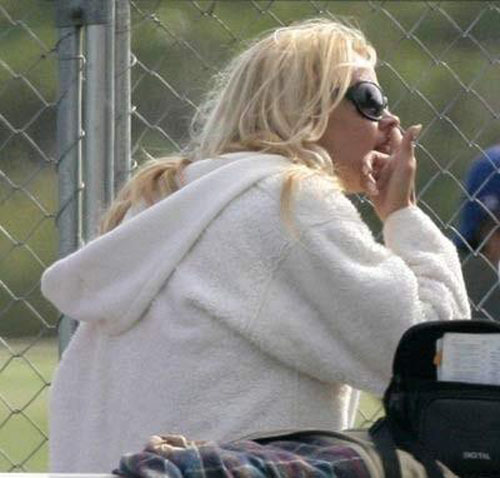
\includegraphics[angle=-2, width=7cm]{L2-Images/nose4.jpg}};}
\uncover<+->{\node at (0,0) {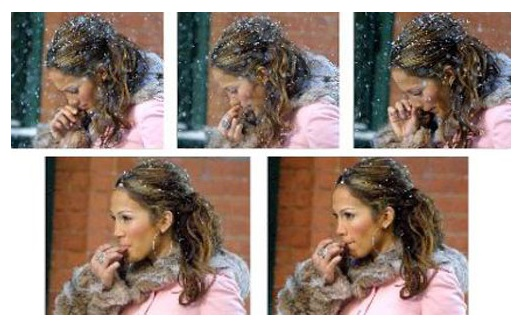
\includegraphics[width=10cm]{L2-Images/nose5.jpg}};}
\end{tikzpicture}
\end{center}
\end{frame}


\begin{frame}
\begin{center}
\begin{huge}
Нельзя публично ковырять в носу!
\end{huge}
\end{center}
\end{frame}

\begin{Person}{freud}{Зигмунд Фрейд}{1856 -- 1939}
\footnotesize{
\begin{tabular}{c c c c}
& \uncover<15->{Ребенок} & \uncover<15->{Взрослый} & \uncover<15->{Родитель} \\
& \uncover<3->{Оно} & \uncover<7->{Я} & \uncover<11->{Сверх-Я} \\
& \uncover<4->{Ид} & \uncover<8->{Эго} & \uncover<12->{Супер-Эго} \\
\uncover<2->{Подсознательное} & \uncover<5->{\normalsize\checkmark} &\uncover<9->{\normalsize\ding{55}} & \uncover<13->{\normalsize\checkmark}\\
\uncover<2->{Сознательное} & \uncover<6->{\normalsize\ding{55}} & \uncover<10->{\normalsize\checkmark} &  \uncover<14->{\normalsize\checkmark}
\end{tabular}}
\end{Person}

\usetikzlibrary{calc}


\begin{frame}
\begin{tikzpicture}[x=3cm,y=-3cm]
\draw (0,0) circle (1);
\uncover<2->{\draw (-1,0) -- node[above] {Нельзя публично ковырять в носу} (1,0);}
\uncover<3->{\node at (0,0.5) {Оно};}
\uncover<4->{\node at (0,-0.5) {Я};} 
\uncover<5->{\draw (-1,0) -- node[below] {Сверх-Я} (1,0);}

\uncover<6>{
\draw[dashed] (-2.5,-0.25) -- node[below] {Бессознательное} (-1,-0.25) -- (1,-0.25);
\draw[dashed] (-2.5,-0.25) -- node[above] {Сознательное} (-1,-0.25) -- (1,-0.25);
}

\uncover<7>{
\draw[dashed] (-2.5,0.25) -- node[below] {Бессознательное} (-1,0.25) -- (1,0.25);
\draw[dashed] (-2.5,0.25) -- node[above] {Сознательное} (-1,0.25) -- (1,0.25);
}
\end{tikzpicture}
\end{frame}

\begin{frame}
\begin{center}
\begin{tikzpicture}[x=1.5cm,y=1.5cm]
\node(n0) at (-2,0) {Можно};
\node(n1) at (2,0) {Нельзя};
\node(n2) at (0,2) {Публично};
\node(n3) at (0,-2) {Непублично};
\draw(n0) -- (n1);
\draw(n2) -- (n3);
\uncover<2->{\node at(1,1) {Автор};}
\uncover<3->{\node[align=center] at(-1,1) {Вытесненная\\ субличность};}
\uncover<4-5>{\node at(1,-1) {Автор};}
\uncover<5>{\node[align=center] at(-1,-1) {Вытесненная\\ субличность};}
\uncover<6->{\node[align=center] at(-1,-1) {Неактуальная\\ субличность};}
\uncover<7>{\node[align=center] at(1,-1) {Бессмыслица};}
\uncover<8>{\node[align=center] at(1,-1) {Вытесненная\\ субличность};}
\end{tikzpicture}
\end{center}
\end{frame}

\begin{frame}
\begin{center}
\begin{small}
\begin{tikzpicture}[x=3cm,y=-1.5cm]
\node (n0) at (0,0) {Нельзя публично ковырять в носу};

\uncover<2->{
\node (n1) at (-1,1) {можно/нельзя};
\node[align=center] (n2) at (0,2) {публично/\\непублично};
\node[align=center] (n3) at (1,1) {ковырять в носу/\\не ковырять в носу};
\draw (n0) -- (n1);
\draw (n0) -- (n2);
\draw (n0) -- (n3);
}
\uncover<3->{
\node[align=center] (n31) at (1,2) {нарушать/не нарушать\\ телесные границы};
\node (n32) at (2,2) {нос/не нос};
\draw (n3) -- (n31);
\draw (n3) -- (n32);
}
\uncover<4->{
\node[align=center] (n11) at (-2,2) {доминирование/\\унижение};
\node[align=center] (n12) at (-1,2) {разрешение/\\запрещение};
\draw (n1) -- (n11);
\draw (n1) -- (n12);
}
\uncover<5->{
\node (n21) at (-2,3) {охранник};
}
\uncover<6->{
\node (n21) at (-1,3) {запрещальщик};
}
\uncover<7->{
\node (n21) at (0,3) {стыдливый};
}
\uncover<8->{
\node (n21) at (1,3) {снежная королева};
}
\uncover<9->{
\node (n21) at (2,3) {цензор};
}
\end{tikzpicture}
\end{small}
\end{center}

\end{frame}

\begin{frame}
Нельзя публично ковырять в носу.
\begin{itemize}
\item<2> Можно публично ковырять в носу
\item<3-> Нельзя ковырять в носу {\bf наедине с собой}
\item<4-> Нельзя публично {\bf не нарушать телесные границы}
\item<5-> Нельзя публично ковырять {\bf не в носу}
\item<6-> {\bf Я обязан} публично ковырять в носу
\item<7-> {\bf Ты не запрещаешь} мне публично ковырять в носу
\end{itemize}
\end{frame}

\begin{frame}

\end{frame}

\end{document}